\chapter{Анализ влияния алгоритма управления приводами СПН и кинематической погрешности привода на величину некомпенсировааных моментов, возникающих при перенацеливании}\label{ch:ch2}
\section{Описание объектов исследования}\label{sec:ch2/sec1}

Одним из объектов исследования является модуль направленного обзора а 
(МНО). Конструкция МНО предусматривает возможность поворота оси 
визирования по двум осям в пределах ограниченного угла. При этом оптическая 
система МНО разделена на две части. В подвижную часть входит зеркальный блок состоящий из главного зеркала  и вторичного зеркала , а неподвижная часть включает линзовый компенсатор,и сканирующее зеркало. Оптические оси этих двух частей составляют угол $90^\circ \pm \beta$, где $\beta$-угол поворота зеркального блока по оси $OZ$ . Зеркальный блок имеет также возможность вращаться по оси $OY$ на угол $\alpha$. Связь частей оптической системы друг с другом осуществляется с помощью плоского сканирующего зеркала 11, развёрнутого относительно оси $ОХ$ на угол $45^\circ \pm \frac{\beta}{2}$.Таким образом, конструктивно подвижная часть установлена в кардане и имеет две степени свободы. Для изменения пространственной ориентации оси визирования МНО


\begin{figure}[ht]
	\begin{minipage}[b][][b]{0.49\linewidth}\centering
	\end{minipage}
	\hfill
	\begin{minipage}[b][][b]{0.49\linewidth}\centering
		\includegraphics[width=1\linewidth]{ypk_cut} \\ б)
	\end{minipage}
	\caption{Система узкопольного канала}
	\label{fig:ypk-pic}
\end{figure}
Изменение пространственной ориентации оси визирования МНО осуществляется за счёт работы специальных приводов, которые поворачивают зеркальный блок относительно космического аппарата на углы $\alpha$ и $\beta$.
Приводы прикладывают к осям карданова подвеса соответствующие моменты для реализации углового перемещения зеркального блока. В соответствии с третьим законом Ньютона, к КА будут приложены равные, но противоположно направленные моменты в месте крепления приводов. Эти моменты называются реактивными.

Реактивные моменты, будучи приложенными к КА, приводят к дополнительному перемещению КА в пространстве, меняя направление оси визирования МНО, закреплённого на КА. Для стабилизации КА в полёте и удержании его на орбите служат гиродины (специальные маховики с приводами или двухстепенные гироскопы). Действие значительных по величине реактивных моментов приводит к существенным нагрузкам на гиродины, и к изначальному угловому положению КА можно вернуться лишь после продолжительного по времени переходного процесса всей системы стабилизации КА.\cite{uglova2019gurodin, zhao2023effect}

В представленной конструкции компенсация реактивного момента реализована за счёт установки маховика на оси двигателя через редуктор. Такое решение одновременно формирует противодействующий момент и обеспечивает автоматическую синхронизацию его вращения с движением нагрузки. При работе привода зеркального блока двигатель через редуктор передаёт вращение как на сам блок, так и на маховик, который разворачивается в противоположную сторону. В результате создаётся момент, равный по величине и противоположный по знаку моменту, приложенному к основанию от движения блока зеркал.Ключевым достоинством выбранной схемы является то, что синхронизация достигается конструктивно, без необходимости в отдельной системе управления маховиком или в алгоритмах согласования его работы с зеркальным блоком. Это существенно упрощает управление и повышает надёжность устройства. Дополнительное преимущество даёт применение редукторной кинематической связи: эквивалентный момент инерции маховика уменьшается пропорционально квадрату коэффициента передачи $i$, что позволяет снизить его массу при сохранении требуемого компенсирующего воздействия. Такой подход делает возможной эффективную компенсацию реактивного момента без значительного увеличения массы и энергопотребления, что особенно важно при проектировании компактных высокоточных приводов.Использование шагового двигателя дополнительно расширяет функциональные возможности конструкции. Так как вращение маховика жёстко связано с движением зеркального блока, управление углом поворота может осуществляться дискретно, по числу шагов двигателя. Это позволяет отказаться от отдельного датчика угла поворота блока зеркал и использовать управление «по шагам» как резервный режим в случае отказа основной системы обратной связи. Такая особенность повышает отказоустойчивость системы при сохранении требуемой точности задания углового положения.

Другим объектом исследования является оптико-механическая система (ОМС), представляющая собой зеркало с двумя степенями свободы.

\begin{figure}[ht] 
	\centerfloat{
		\includegraphics[scale=0.8]{zerkalo} 
	}
	\legend{1 – оптико-механическое устройство; 2 – рама несущая; 3 – привод редукторный OY; 4 – узел датчика угла; 5 – узел привода редукторного OZ; 6 – привод редукторный OZ; 7 – арретир технологический; 8 – технологический электронный блок управления ПЭС}
	\caption{Оптическая система Зеркало.}
	\label{fig:zerkalo} 
\end{figure}

Изделие, показанное на рисунке~\cref{fig:zerkalo}, представляет собой оптико-механическое устройство (ОМУ) (1) с поворотной электромеханической системой (ПЭС) и технологическим электронным блоком управления ПЭС (8), которые обеспечивают:
\begin{itemize}[beginpenalty=10000] % https://tex.stackexchange.com/a/476052/104425
	\item угловые перемещения ОМУ по двум координатам, позволяющие осуществить вращение линии визирования ОС;
	\item высокую точность перенацеливания;
	\item малое значение остаточных реактивных моментов, действующих на основание при перенацеливании изделия;
	\item фиксирование пространственного положения линии визирования после завершения перенацеливания;
	\item формирование сигналов оперативного и телеметрического контроля (ОК и ТМ);
	\item стойкость к внешним воздействующим факторам.
\end{itemize}

ОМУ (1) изделия состоит из зеркала, системы крепления и оси для установки в изделие.Зеркало выполнено из бериллия, имеет монолитную конструкцию с шестигранными облегчающими выборками, гнездом под систему крепления и отверстия для размещения оси. Плоская рабочая поверхность зеркала сформирована оптической обработкой непосредственно бериллиевой поверхности без применения дополнительного зеркального покрытия.

Система крепления и ось вращения обеспечивают надёжное крепление зеркала в ПЭС.

Конструктивно в состав ПЭС входят:
\begin{itemize}[beginpenalty=10000] % https://tex.stackexchange.com/a/476052/104425
	\item рама несущая (2);
	\item привод редукторный \textit{OZ} (3);
	\item узел датчика угла (4);
	\item узел привода редукторного \textit{ОY} (5);
	\item формирование сигналов оперативного и телеметрического контроля (ОК и ТМ);
\end{itemize}
Рама несущая (2) представляет собой жёсткую конструкцию в виде несущих опор, предназначенную для крепления всех составных частей изделия.

Привод редукторный \textit{OZ} (3) поворачивает зеркало ОМУ (1) вокруг вертикальной оси \textit{OZ}, обеспечивая перенацеливание по азимуту на углы до $\pm10^{\circ}$ . 
В состав привода редукторного \textit{OZ} входят два шаговых двигателя (основной и резервный) с волновым редуктором и маховиком.
Шаговые двигатели соединены друг с другом зубчатой передачей с коэффициентом передачи 1.

Каждый двигатель имеет два выходных вала с противоположных сторон двигателя. На один вал основного двигателя крепится маховик. На другой, через муфту и ось, – волновой редуктор, предназначенный для передачи вращения от шагового двигателя к системе крепления зеркала ОМУ (1). При этом выходной вал волнового редуктора вместе с зеркалом ОМУ вращается в направлении, обратном вращению валов основного двигателя, что обеспечивает вращение маховика в направлении, обратном вращению зеркала, и компенсацию момента, приложенного к основанию, возникающего при вращении зеркала.

К приводу редукторному \textit{OZ} крепится узел датчика угла (4), включающий преобразователь угловых перемещений, передающий информацию о текущем угле поворота зеркала по азимуту (вокруг оси \emph{OZ}).
Узел привода редукторного \emph{OY} (5) является подвижной частью изделия. В его состав входит поворотная несущая конструкция, состоящая из пластин и кронштейнов, с закреплённым на ней приводом редукторным \emph{OY} (6). 

Привод редукторный \emph{OY} поворачивает зеркало ОМУ вокруг горизонтальной оси \emph{OY}, обеспечивая перенацеливание по углу места на углы до $\pm10^{\circ}$. 

Узел датчика угла (4), установленный на оси ОМУ (1) с противоположной стороны от привода редукторного OY (6), обеспечивает измерение угла поворота зеркала по углу места (вокруг оси \emph{OY}).

Конструктивно привод редукторный \emph{OY} (6) и привод редукторный \emph{OZ} (3) выполнены одинаково и отличаются только маховиками. Конструкция датчиков угла, установленных по осям \emph{OY} и \emph{OZ}, также одинакова.

В составе изделия узел привода редукторного \emph{OY} обеспечивает также крепление ОМУ (1) и привода редукторного \emph{OZ} (3), и с помощью последнего вращается вокруг оси \emph{OZ} относительно рамы несущей (2). При этом привод редукторный \emph{OZ} (3) остаётся неподвижным, а привод редукторный \emph{OY} (6) разворачивается вместе с узлом привода редукторного \emph{OZ} (5) и зеркалом ОМУ. 

Технологический электронный блок управления (ТЭБУ) ПЭС (8) предназначен для управления ПЭС изделия по командам, поступающим извне от автоматизированной системы контроля и управления (АСКУ) в составе технологического стенда проверки основных параметров ПЗС ОМС.


\section{Математическое описание реактивных моментов, возникающих при перенацеливании оптической системы МНО}\label{sec:ch2/sec2}

Особенностью конструкции МНО является несовпадение точки пересечения осей карданова подвеса с центром тяжести подвижного зеркального блока (Рисунок ~\cref{fig:tikz_YPK}).
Обозначим расстояние между этими точками за $r$. 

Рассмотрим результат воздействия реактивных моментов на основание с учётом расположения центра вращения карданова подвеса МНО относительно центра тяжести КА.
\begin{figure}[ht]
	\centerfloat{
		\ifdefmacro{\tikzsetnextfilename}{\tikzsetnextfilename{tikz_example_compiled}}{}% присваиваемое предкомпилированному pdf имя файла (не обязательно)
		
	\begin{tikzpicture}[scale=1.6, >=stealth, font=\small]
		%X0Y0Z0 axis
		\draw [->, very thick] (13.75,13.25) -- (13.75,16.25)node[above] {$Y_0$};
		\draw [->, very thick] (13.75,13.25) -- (11.5,11.5) node[above] {$X_0$};
		\draw [->,very thick] (13.75,13.25) -- (11.25,13.75) node[above] {$Z_0$};
		\node at (13.85, 13.15) {$0_0$};
		%Z0 line
		\draw [thin, short] (11.25,13.75) -- (16.25,12.75);
		%Z line
		\draw [thin, short] (13.75,13.25) -- (16.75,13);
		
		%X0Y0Z0 axis proection
		\draw [thin] (10,8.25) -- (10,10.75) node[above] {$Y_0$};
		\draw [thin] (10,8.25) -- (7.5,8.75) node[above] {$Z_0$};
		\draw [thin] (10,8.25) -- (7.5,6.5) node[above] {$X_0$};
		
		
		%proection Z0 line
		\draw [thin, short] (7.5,8.75) -- (12.5,7.75);
		\draw [line width=0.9pt, ->,] (10,8.25) -- (10,10) node[right] {$Mda$};
		%OXYZ axis
		\draw [ ->, very thick] (10,8.25) -- (9.75,6.25) node[left] {$X$};
		\draw [->, very thick] (10,8.25) -- (9.32, 10.2) node[above] {$Y$};
		\draw[thick,->] (10, 10) arc[start angle=5,end angle=175,x radius=0.3cm, y radius=0.2cm];
		\node at (9.7, 10.3) {$\beta$};
		\draw [ ->, very thick] (10,8.25) -- (7,8.5) node[above] {$Z$};
		\node at (10.15,8.35) {$0$};
		\draw[thick,->] (8.8,8.5) arc[start angle=0,end angle=85,radius=-1.2cm];
		\node at (9.5, 7.5) {$\alpha$};
		%red line
		\draw [ color={rgb,255:red,245; green,0; blue,0}, line width=1.6pt, short] (13.75,13.25) -- (10,8.25);
		\node at (11, 10)[text=red] {$R$};
		\draw [ color=red, line width=0.2pt, ->,] (10,8.25) -- (9.75,9)node[left] {$Fb$};
		
		
		
		\draw [line width=0.9pt, ->,] (10,8.25) -- (7.8,8.43) node[above] {$Mdb$};
		\draw [ color=red, line width=0.2pt, ->,] (10,8.25) -- (8.5,8.37) node[above] {$Fa$};
		%blue circle
		\draw [ color={rgb,255:red,4; green,45; blue,251} , fill={rgb,255:red,45; green,166; blue,240}, line width=0.2pt ] (9.83,7) circle (0.25cm);
		
		
		
		\draw [ color=blue, very thick, short] (10,8.25) -- (9.83,7);
		\node at (10, 7.5)[text=blue] {$r$};
		\end{tikzpicture}
		
	}
	\legend{}
	\caption[Пример \texttt{tikz} схемы]{Смещение центра масс блока зеркал МНО}\label{fig:tikz_YPK}
\end{figure}

Свяжем с центром масс КА $O_0$  неподвижную систему координат $О_0X_0Y_0Z_0$. С центром карданова подвеса свяжем систему координат $ОXYZ$, развёрнутую относительно неподвижной системы координат на углы $\alpha$ и $\beta$. Редукторный привод карданова подвеса, установленный на оси $ОY_0$, неподвижен, а второй редукторный привод, установленный на оси $OZ$, имеет возможность разворачиваться на угол $\alpha$ вместе с внутренней рамой карданова подвеса. 

Узел зеркал неуравновешен относительно внутренней оси карданова подвеса. Центр масс узла зеркал $O_1$ смещён относительно центра карданова подвеса на расстояние $r$. Центр карданова подвеса $O$ имеет координаты $R_x$,$R_y$,$R_z$ в неподвижной системе координат $О_0X_0Y_0Z_0$. Для разворота узла зеркал на углы $\alpha$ и $\beta$ по соответствующим осям создаются моменты $M_{da}$ и $M_{db}$ при помощи приводов. Эти моменты одновременно приводят в движение компенсационные маховики приводов и узел зеркал. В свою очередь, узел зеркал (с подвижными элементами карданова подвеса) имеет собственные моменты инерции $J_da$ и $J_db$ относительно осей, связанных с центром карданова подвеса. К центру масс узла зеркал будут приложены силы $F_a$ и $F_b$, приводящие узел зеркал в движение, тогда к основанию КА в точке, соответствующей центру карданова подвеса, будут приложены силы $F_a$ и $F_b$, направленные в противоположную сторону.

Если центр масс КА (точка $O_0$) и центр карданова подвеса (точка $O$) не совпадают, то к КА будут приложены реактивные моменты, вызванные силами $F_a$ и $F_b$. С другой стороны, двигатели приводов приводят во вращение маховики, что сопровождается возникновением  соответствующих моментов $M_{ma}$ и $M_{mb}$ реакции на КА. Результирующие реактивные моменты можно рассчитать как сумму всех перечисленных воздействий.

Сканирующее зеркало связано кинематически с зеркальным блоком через рычажный механизм, который с высокой точностью делит угол поворота $\beta$ зеркального блока на 2 и поворачивает сканирующее зеркало на угол $\beta/2$ вокруг оси $OZ$. Поэтому момент инерции сканирующего зеркала может быть включён в момент инерции $J_{db}$.

Таким образом, к основанию приложены реактивные моменты, некоторые из которых можно представить в виде соответствующих пар сил:\\

\begin{samepage}
	\begin{equation}
		\label{eq:eq_Mra}
		\begin{alignedat}{2}
			M_{ra} &= F_a r + M_{da} - M_{ma}
		\end{alignedat}
	\end{equation}
	\begin{equation}
		\label{eq:eq_Mrb}
		\begin{alignedat}{2}
			M_{rb} &= F_b r + M_{db} - M_{mb}
		\end{alignedat}
	\end{equation}
	
	\begin{align*}
		\text{где}     			& \quad M_{da}= \epsilon_{da}J_{da};\\           
		& \quad F_a= \frac{M_{da}-M_{ma}}{r};        \\
		& \quad F_b = \frac{M_{db}-M_{mb}}{r}; \\
		& \quad J_{ma}, J_{mb} - \textnormal{моменты инерции компенсационных маховиков, установленных по осям $O_1Y_0$ и $O_1Z$}         \\
		& \quad \epsilon_{da}, \epsilon_{db} -\textnormal{ углы ускорения подвижных частей карданова подвеса по соответствующим углам поворота}          \\
		& \quad \epsilon_{ma}, \epsilon_{mb} - \textnormal{угловые ускорения подвижных частей карданова подвеса по соответствующим углам поворота}
	\end{align*}
\end{samepage}

Спроецируем силы $F_a$ и $F_b$, приложенные к центру карданова подвеса, на оси неподвижной системы координат $O_0X_0Y_0Z_0$:
\begin{samepage}
	\begin{equation}
		\label{eq:eq_F0_proect}
		\begin{aligned}
			F_{X_0} &= F_a\sin(\alpha)+F_b\sin(\beta)\cos(\alpha) \\
			F_{Y_0} &=F_b\cos(\beta) \\
			F_{Z_0} &= F_a\cos(\alpha)-F_b\sin(\alpha)\sin(\beta)
		\end{aligned}	
	\end{equation}
\end{samepage}

Нетрудно показать, что эти силы, приложенные к КА в точке $O$, создадут моменты относительно центра масс $O_0$. С учётом ~\cref{eq:eq_Mra, eq:eq_Mrb} для проекций момента возмущения на оси КА получим:
\begin{samepage}
	\begin{equation}
		\label{eq:eq_M_proect}
		\begin{aligned}
			M_{X_0} &= F_{Z_0}R_Y+F_{Y_0}R_Z+(M_da-M_ma)\sin(\alpha) \\
			M_{Y_0} &= F_{X_0}R_Z+F_{Z_0}R_X+(M_da-Mma)\\
			M_{Z_0} &= F_{Y_0}R_X+(M_db-M_mb)\cos(\alpha)
		\end{aligned}	
	\end{equation}
\end{samepage}

Подставим проекции сил из уравнения ~\cref{eq:eq_F0_proect} в ~\cref{eq:eq_M_proect}, получим:
\begin{samepage}
	\begin{equation}
		\label{eq:eq_M_proect_F}
		\begin{aligned}
			M_{X_0} &= F_a\cos(\alpha)-F_b\sin(\alpha)\sin(\beta)R_Y+F_{Y_0}R_Z+(M_{da}-M_{ma})\sin(\alpha) \\
			M_{Y_0} &= F_a\sin(\alpha)+F_b\sin(\beta)\cos(\alpha)R_Z+F_{Z_0}R_X+(M_{da}-M{ma})\\
			M_{Z_0} &= F_b\cos(\beta)R_X+(M_{db}-M_{mb})\cos(\alpha)
		\end{aligned}	
	\end{equation}
\end{samepage}

В выражении ~\cref{eq:eq_M_proect_F} проекции моментов на оси состоят их суммы двух частей моментов, возникающих от смещения центра карданова подвеса относительно центра масс КА (слагаемые, содержащие $R_X$,$R_Y$,$R_Z$), и моментов, возникающих из-за неполной компенсации моментов двигателей моментами соответствующих маховиков. 



\section{Пример расчёта остаточных реактивных моментов на основание}\label{sec:ch2/sec2}

$M_{X_0}$, $M_{Y_0}$, $M_{Z_0}$ – суммарные значения реактивных моментов, действующих на КА по соответствующим осям, – рассчитываются по следующим выражениям:

\begin{samepage}
	\begin{equation}
		\label{eq:eq_M_sum}
		\begin{aligned}
			M_{X_0}&=M_{X_c}+M_{X_1} \\
			M_{Y_0}&=M_{Y_c}+M_{Y_1} \\
			M_{Z_0}&=M_{Z_c}+M_{Z_1} \\
		\end{aligned}	
	\end{equation}
	
	\begin{align*}
		\text{где} \quad
		M_{X_c} &= \left(F_a \cos(\alpha) - F_b \sin(\alpha) \sin(\beta)\right) R_Y + F_B \cos(\beta) R_Z, \\
		M_{Y_c} &= \left(F_a \sin(\alpha) - F_b \sin(\beta) \cos(\alpha)\right) R_Z + \left(F_a \cos(\alpha) + F_b \sin(\alpha) \sin(\beta)\right) R_X, \\
		M_{Z_c} &= F_b \cos(\beta) R_X
	\end{align*}
\end{samepage}

Моменты $M_{Xc}$, $M_{Yc}$, $M_{Zc}$ возникают из-за смещения центра масс КА относительно центра карданова подвеса на величины $R_x$, $R_y$, $R_z$ соответственно.
\begin{equation}
	\label{eq:eq_M1_proect}
	\begin{aligned}
		M_{X_1}&=(M_{db}-M_{mb})\sin(\alpha) \\
		M_{Y_1}&=M_{da}-M_{ma} \\
		M_{Z_1}&=M_{db}-M_{mb}\cos(\alpha) \\
	\end{aligned}	
\end{equation}
Моменты $M_{X1}$, $M_{Y1}$, $M_{Z1}$, возникают из-за неполной компенсации реактивных моментов маховиками.

Для расчёта остаточных реактивных моментов зададимся следующими значениями параметров (Таблица~\cref{tab:unit:init_data})

\begin{table}
	\centering
	\begin{threeparttable}
		\caption{Исходные данные}
		\label{tab:unit:init_data}
		\begin{tabular}{llc}
			\toprule
			Параметр                  & Значение              & Размерность             \\
			\midrule
			$J_a$                     & 2,84           			& \si{\text{кг}.\text{м}^2}            \\
			$J_b$                     & 1,9      				& \si{\text{кг}.\text{м}^2}        \\
			$\varepsilon_\alpha$	  & 0,127					&
			\si{\text{рад}/\text{с}^2}   \\
			$\varepsilon_\beta$		  & 0,127					&
			\si{\text{рад}/\text{с}^2} \\
			$r$                       & 0,3          			& \si{\text{м}}           \\
			$R_X$                     & 1,212          			& \si{\text{м}}           \\
			$R_Y$                     & 0,28  					& \si{\text{м}}   \\
			$R_Z$                     & 0,015         			& \si{\text{м}}          \\
			$J_{ma}$                  & 0,0169                	& \si{\text{кг}.\text{м}^2}           \\
			$J_{mb}$                  & 0,0113              	& \si{\text{кг}.\text{м}^2}           \\
			$\alpha$                  & 0,0873                     	& \si{\text{рад}}          \\
			$\beta$                   & 0,0873                     	& \si{\text{рад}}          \\
			\bottomrule
		\end{tabular}
	\end{threeparttable}
\end{table}

Пользуясь формулами ~\eqref{eq:eq_Mra}-\eqref{eq:eq_M1_proect} и исходными данными таблицы ~\cref{tab:unit:init_data}, получим расчётные значения параметров (таблицы ~\cref{tab:unit:calcData1} и ~\cref{tab:unit:resultData}).


\begin{table}
	\centering
	\begin{threeparttable}
		\caption{Расчётные значения}
		\label{tab:unit:calcData1}
		\begin{tabular}{llc}
			\toprule
			Параметр             		& Значение              & Размерность             		\\
			\midrule
			$M_{da}$                & 0,3607          		& \si{\text{H}.\text{м}}          \\
			$M_{db}$                & 0,2413  				& \si{\text{H}.\text{м}}   \\
			$F_a$                   & 0,0504         		& \si{\text{H}}         \\
			$F_b$                  	& 0,0378                & \si{\text{H}}          \\
			$F_{X_0}$                  	& 0,0077              	& \si{\text{H}}           \\
			$F_{Y_0}$                  	& 0,0377                & \si{\text{H}}          \\
			$F_{Z_0}$                   & 0,0499                & \si{\text{H}}          \\
			\bottomrule
		\end{tabular}
	\end{threeparttable}
\end{table}

\begin{table}
	\centering
	\begin{threeparttable}
		\caption{Результаты расчёта}
		\label{tab:unit:resultData}
		\begin{tabular}{llc}
			\toprule
			Параметр             		& Значение              & Размерность             		\\
			\midrule
			$M_{Xc}$       				& 0,0145      			& \si{\newton\metre}      			\\
			$M_{Yc}$         			& 0,0606           		& \si{\newton\metre}          	\\
			$M_{Zc}$            		& 0,0456          		& \si{\newton\metre}           				\\
			$M_{X_1}$                   & 0,0013           		& \si{\newton\metre}            		\\
			$M_{Y_1}$            		& 0,0151      			& \si{\newton\metre}       \\
			$M_{Z_1}$            		& 0,0113      			& \si{\newton\metre}      \\
			$M_X$            			& 0,0158          		& \si{\newton\metre}    \\
			$M_Y$                		& 0,0757          		& \si{\newton\metre}          \\
			$M_Z$                		& 0,0569  				& \si{\newton\metre}   \\
			
			\bottomrule
		\end{tabular}
	\end{threeparttable}
\end{table}


\begin{figure}[ht]
	\centerfloat{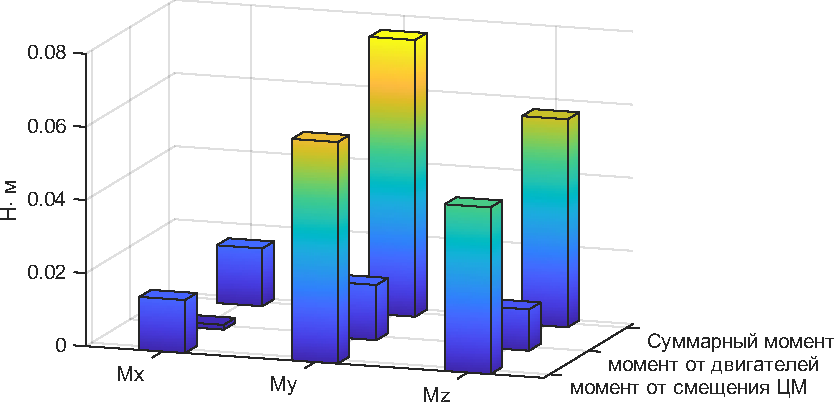
\includegraphics[scale=0.7]{matlab/moments_chart.pdf}}
	
	\caption{Распределение моментов по осям $Mx$, $My$, $Mz$ для различных источников воздействия: смещения центра масс, действия двигателей и их суммарного эффекта}
	\label{fig:momentBars}
\end{figure}

На рисунке ~\cref{fig:momentBars} приведено графическое изображение полученных результатов.

Таким образом, при заданных параметрах основной вклад в реактивные моменты вносит смещение центра карданова подвеса относительно центра масс КА, поэтому при компоновке КА указанное смещение должно быть минимизировано.

Итак, на основании изложенного можно сделать вывод о том, что максимальные реактивные моменты, действующие на основание со стороны редукторных приводов во время их функционирования, для представленного набора исходных данных не превышают величину 0,1 \si{\newton\metre}.  Основной вклад в эти моменты вносят составляющие, возникающие от наличия смещения центра карданова подвеса УПК относительно центра масс КА.

С помощью добавочных колец можно подобрать моменты инерции маховиков с целью уменьшения влияния реактивных моментов на КА.

\section{Анализ влияния остаточного реактивного момента на параметры качества изображения}

На основе параметров, рассчитанных в предыдущей главе, был изготовлен лётный образец ОМУ, интегрированный в состав космического аппарата. После выведения на орбиту с бортовых гироскопов были собраны данные об угловых скоростях спутника. Эти данные послужили исходной информацией для последующего анализа воздействия остаточного реактивного момента на качество изображений. на рисунке ~\cref{fig:sat_gyro_data} представлены данные бортовых гироскопов, показывающие угловые скорости спутника за длительный период времени. В целом они отражают работу системы ориентации в штатном режиме.

\begin{figure}[h]
	\centering
	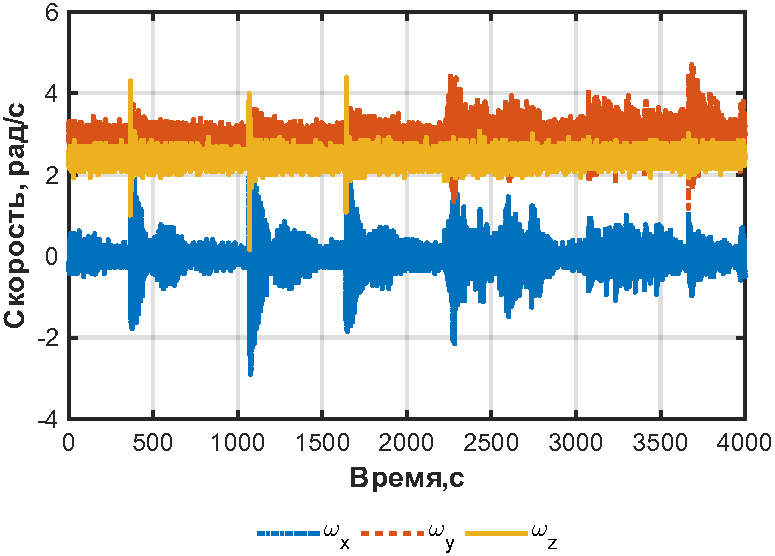
\includegraphics[width=0.8\linewidth]{matlab/img/sat_gyro_data.pdf}
	\caption{Данные бортовых гироскопов}
	\label{fig:sat_gyro_data}
	\end{figure}

Для анализа были выделены интервалы, в которых ось визирования поворачивалась на максимально возможные углы. Именно в эти моменты реактивные моменты достигают наибольших значений. Графики угловых скоростей при повороте оси визирования представлены на рисунке ~\cref{fig:rotationYZ}.

\begin{figure}[h]
	\begin{minipage}[b][][b]{0.49\linewidth}\centering
		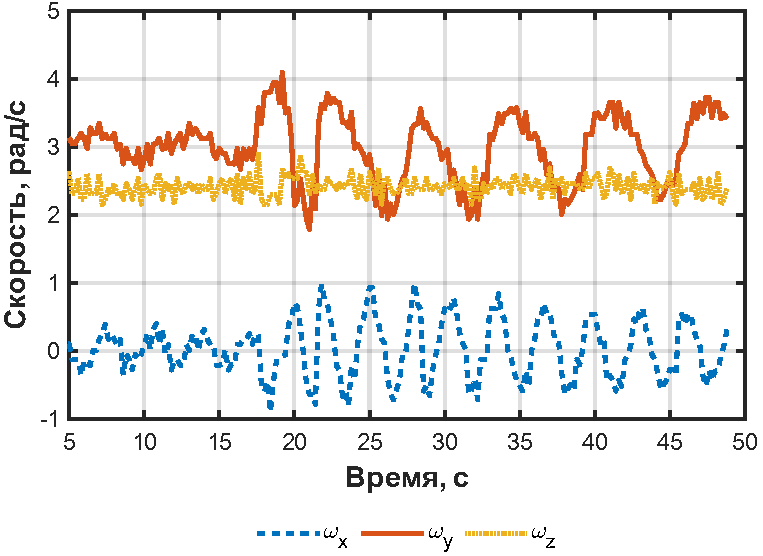
\includegraphics[width=1\linewidth]{matlab/img/sat_gyro_dataY.pdf} \\ a)
	\end{minipage}
	\hfill
	\begin{minipage}[b][][b]{0.49\linewidth}\centering
		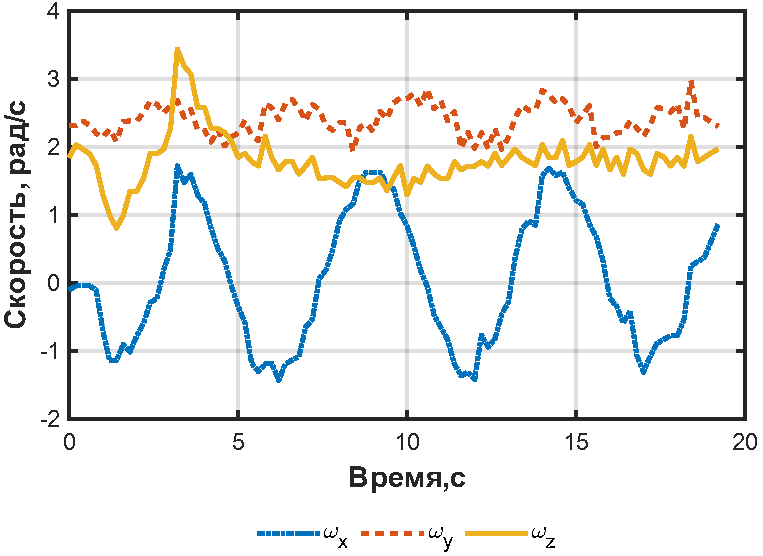
\includegraphics[width=1\linewidth]{matlab/img/sat_gyro_dataZ.pdf} \\ б)
	\end{minipage}
	\caption{Скорость угловых колебаний спутника при повороте оси визирования по a) оси $OY$, б) оси $OZ$ }
	\label{fig:rotationYZ}
\end{figure}

Так как ось $OX$ совпадет с оптической осью -- вращение вокруг $OX$ не приводит к параллельному смещению изображения и, соответственно, не формирует линейный \blur{}. Поэтому по измеренным угловым скоростям были получены и использованы углы $\theta_y$, $\theta_z$, отвечающие за трансляцию изображения в плоскости фокуса.

\begin{equation}
	\label{eq:thetaZY}
	\theta_{y,z}(t)= \int \omega_{x,y}\, dt
\end{equation}

\begin{figure}[!h]
	\begin{minipage}[b][][b]{0.49\linewidth}\centering
		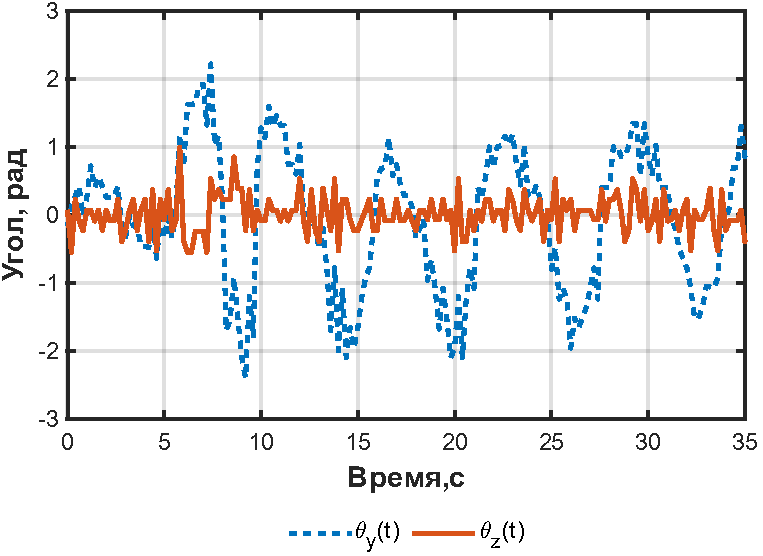
\includegraphics[width=1\linewidth]{matlab/img/thetaY.pdf} \\ a)
	\end{minipage}
	\hfill
	\begin{minipage}[b][][b]{0.49\linewidth}\centering
		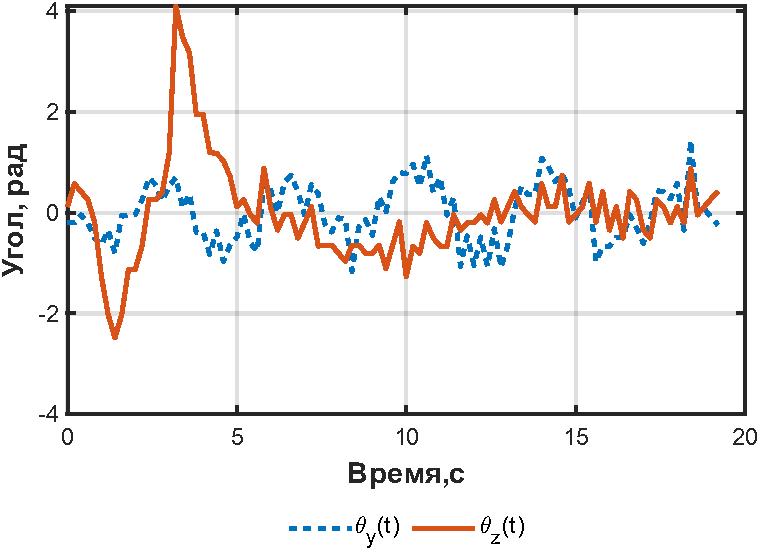
\includegraphics[width=1\linewidth]{matlab/img/thetaZ.pdf} \\ б)
	\end{minipage}
	\caption{Угловое перемещение спутника при повороте оси визирования по a) оси $OY$, б) оси $OZ$ }
	\label{fig:theta}
\end{figure}

\begin{samepage}
Смещение изображения в фокальной плоскости определяется по формуле ~\eqref{eq:bias}, график показан на рисунке ~\ref{fig:bias}

\begin{equation}
	\label{eq:bias}
	\mathbf{r}(t) = 
	\begin{bmatrix}
		y(t) \\
		z(t) \\
	\end{bmatrix}
	= f \cdot
	\begin{bmatrix}
		\theta_{y}(t) \\
		\theta_{z}(t)
	\end{bmatrix}
\end{equation}

где \(f=900000\) мкм --- фокусное расстояние
\end{samepage}

\begin{figure}[ht]
	\begin{minipage}[b][][b]{0.49\linewidth}\centering
		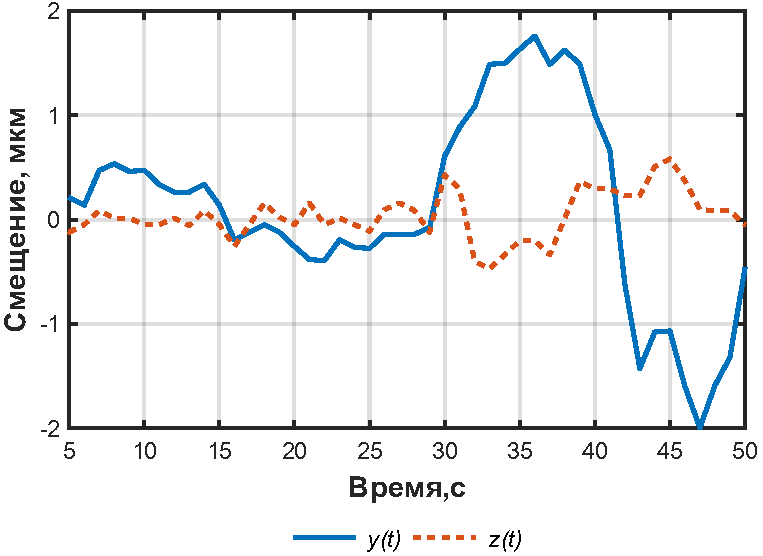
\includegraphics[width=1\linewidth]{matlab/img/biasY.pdf} \\ a)
	\end{minipage}
	\hfill
	\begin{minipage}[b][][b]{0.49\linewidth}\centering
		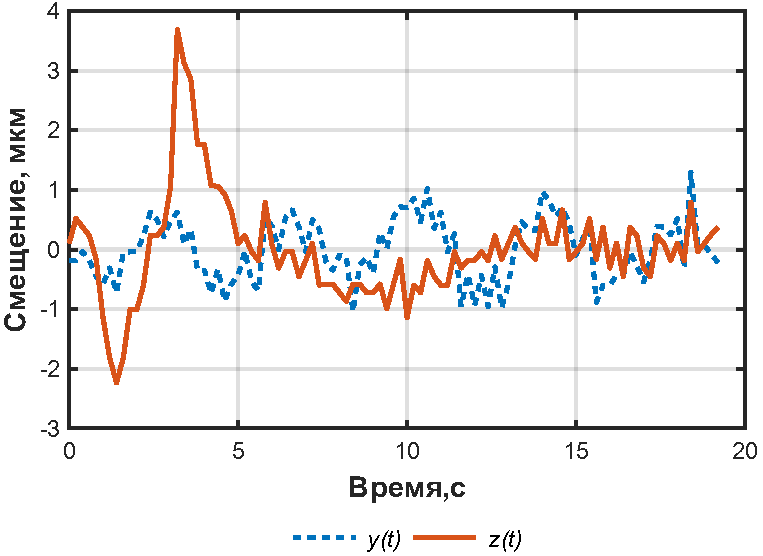
\includegraphics[width=1\linewidth]{matlab/img/biasZ.pdf} \\ б)
	\end{minipage}
	\caption{Смещение в фокальной плоскости при повороте оси визирования по a) оси $OY$, б) оси $OZ$ }
	\label{fig:bias}
\end{figure}


За время экспозиции результирующий сдвиг характеризуется длиной

\begin{equation}
	\label{eq:biasL}
	L=\sqrt{(\Delta x)^2+(\Delta y)^2}
\end{equation}

\begin{figure}[!h]
	\begin{minipage}[b][][b]{0.49\linewidth}\centering
		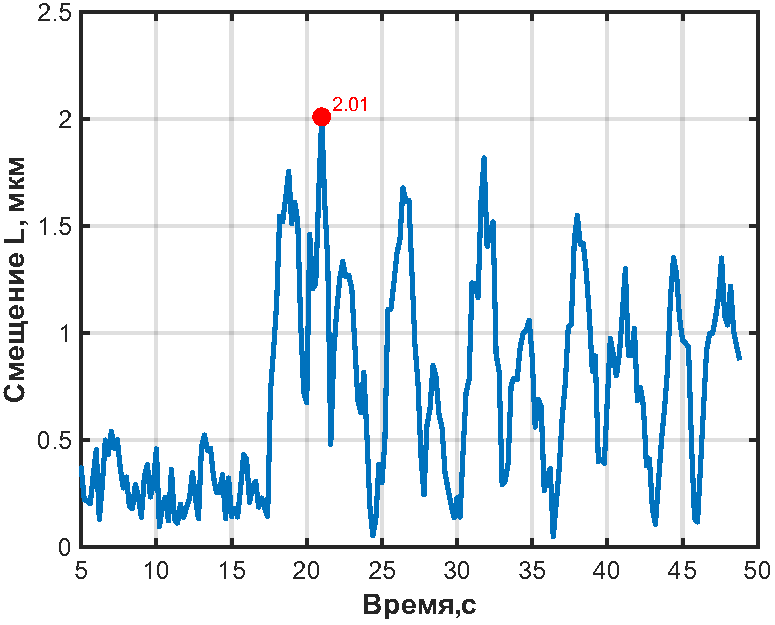
\includegraphics[width=1\linewidth]{matlab/img/LmaxY.pdf} \\ a)
	\end{minipage}
	\hfill
	\begin{minipage}[b][][b]{0.49\linewidth}\centering
		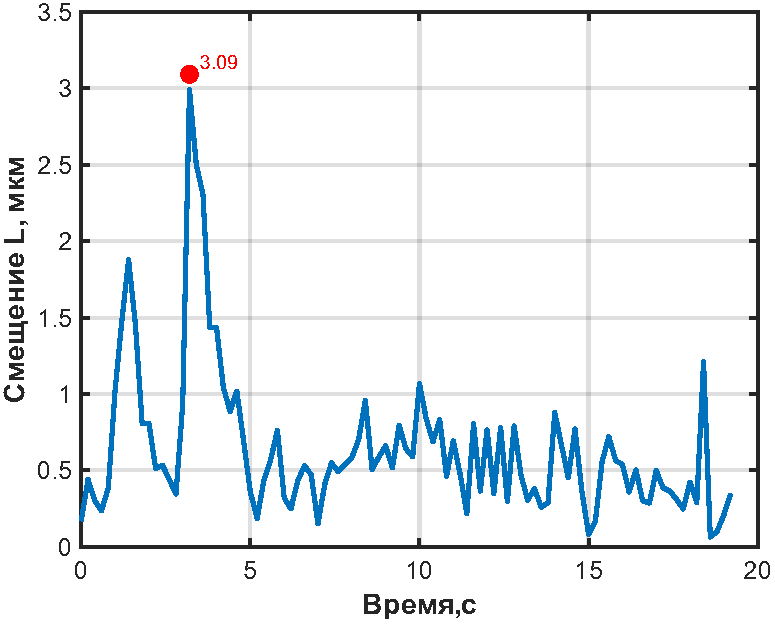
\includegraphics[width=1\linewidth]{matlab/img/LmaxZ.pdf} \\ б)
	\end{minipage}
	\caption{Полное смещение в фокальной плоскости при повороте оси визирования по a) оси $OY$, б) оси $OZ$ }
	\label{fig:biasL}
\end{figure}

Траектория сдвига в пределах экспозиции квазипрямолинейна, поэтому деградация ФПМ вдоль худшего направления описывается аппроксимацией линейного размытия:

\begin{equation}
	\label{eq:MTF_aprox}
  MTF(\nu) = \frac{\sin\!\bigl(\pi \nu L\bigr)}{\pi \nu L}
	\end{equation}

где \(\nu\) -- частота Найквиста по дискретизации, определяется по формуле ~\eqref{eq:nykvist}

\begin{equation}
	\label{eq:nykvist}
	\nu = \frac{1}{2p} \approx \SI{16.7}{\per\milli\meter}
\end{equation}
где \(p\) --- размер пикселя, в исследуемой системе составляет \SI{30}{\micro\meter}

Согласно рассчитанным траекториям (см. рисунок ~\ref{fig:biasL}), максимальная величина результирующего смещения изображения за время экспозиции:
\begin{enumerate}
	\item поворот вокруг $OY$: $L= \SI{2,01}{\micro\meter}$
	\item поворот вокруг $OZ$: $L= \SI{3,74}{\micro\meter}$
	\end{enumerate}
	
В относительных единицах это соответствует:
\begin{equation}
	\frac{L_{OY}}{p} \approx 0,67 \quad \quad \frac{L_{OZ}}{p} \approx 0,124
\end{equation}

На предельной частоте дискретизации $\nu = \nu_N$ получаем:

\begin{equation}
	\begin{split}
	\label{eq:MTF_result}
	MTF(\nu_N)_{OY}=\frac{\sin\!\bigl(\pi \nu_N L\bigr)}{\pi \nu_N L} =  \frac{\sin\!\bigl(\pi 16,7 0,00201 \bigr)}{\pi 16,7 0,00201} \approx  0,9981\\
	MTF(\nu_N)_{OZ}=\frac{\sin\!\bigl(\pi \nu_N L\bigr)}{\pi \nu_N L} =  \frac{\sin\!\bigl(\pi \cdot 16,7 \cdot 0,00374 \bigr)}{\pi \cdot 16,7 \cdot 0,00374} \approx 0,9936
	\end{split}
	\end{equation}

Расчётные значения показали, что при действии остаточного реактивного момента смещение изображения в фокальной плоскости составляет не более 0,13 пикселя. Оценка функции передачи модуляции подтверждает, что деградация на предельной частоте Найквиста не превышает 1 \%, что соответствует современным требованиям к качеству изображения.




Таким образом, с точки зрения \blur воздействие остаточного реактивного момента не является критичным, что подтверждает достоверность предварительного кинематического расчёта. Однако, данные анализа указывают на наличие длительных незатухающих колебаний после манёвра. Эти колебания не приводят к заметному размытию изображения, но создают значительную нагрузку на систему стабилизации космического аппарата и ухудшают её долговременную точность. 

Для снижения уровня колебаний необходимо совершенствование системы управления приводами. В частности, требуется выбор оптимального профиля разгона и торможения двигателей. Для этого был проведён спектральный анализ колебаний КА (рисунок ~\cref{fig:specrtumSat})

%todo описание спектрального анализа

На основе проведённого анализа можно заключить, что для обеспечения устойчивой работы требуется создание специализированного стенда для измерения остаточного реактивного момента. Такой стенд позволит проводить наземную отработку, объективно оценивать воздействие приводов на основание и отрабатывать методы балансировки и компенсации до проведения лётных испытаний. При этом, помимо исследуемой оптической системы планируется использование других конструктивных решений, в которых компенсация осуществляется отдельным двигателем. В подобных случаях необходимо эмпирическое согласование вращения двигателя нагрузки и компенсирующего двигателя, что тоже должно быть обеспечено в рамках стендовых испытаний.

Для выбранных интервалов, соответствующих поворотам оси визирования по осям $OY$ и $OZ$, были рассчитаны значения смещения изображения $\alpha$ за время экспозиции $\tau_{exp}$ 

\begin{equation}
	\alpha(t)=v(t)\cdot \tau_{exp}
\end{equation}

Таким образом, по каждой из осей были получены временные ряды, характеризующие фактическое смещение изображения на матрице при поворотах визирной оси.

%todo рисунки

Влияние \blur{} на пространственные характеристики изображения оценивались через функцию передачи модуляции, задаваемую выражением:

\begin{equation}
	MTF(v) = \frac{\sin\!\bigl(\pi \alpha v\bigr)}{\pi \alpha v}
\end{equation}

где \(v\) --- пространственная частота, \(\alpha\) --- величина смещения изображения в плоскости приёмника.

Эта зависимость отражает ухудшение контрастной передачи системы при относительном движении изображения и служит стандартной моделью при расчёте интегральных показателей качества изображения. \cite{pratt2007digital}.

Расчеты ФПМ 
%todo формулы мтф по осям



\section{Синусоидальный алгоритм управления}\label{sec:ch2/sec1}

Рассмотрим алгоритм управления при котором угловое ускорения привода меняется по закону синуса:

\begin{samepage}
	\begin{equation}
		\label{eq:eqCh2_sin}
		\begin{aligned}
			\epsilon = U \cdot \sin(f \cdot t)
		\end{aligned}	
	\end{equation}
	где \( U \) "--- амплитуда ускорения, \( f \) "--- круговая частота, \( T \) "---период поворота.
\end{samepage}
	
Тогда, интегрируя это выражение, получим для угловой скорости:
\begin{equation}
	\label{eq:eqCh2_sinIntegral}
	\Omega = \left(1 - \cos\left(f \cdot t\right)\right) \cdot \frac{U}{f} \quad \si{\radian\second}
\end{equation}

Проинтегрировав ещё раз - получим выражение для угла поворота:
\begin{equation}
	\label{eq:eqCh2_sinIntegral2}
	\phi = \left( \frac{t}{f} - \sin\left(f \cdot t\right) \right) \cdot \frac{U}{f^2} \si{\radian}
\end{equation}

Из условия, что время перемещения подвижной части $T = 4 \si{\sec}$, угол поворота выходного вала равен $\phi = \SI{17}{\degree} = \SI{0.297}{\radian}$.
Из уравнения ~\cref{eq:eqCh2_sinIntegral2} получим:

\begin{equation}
	\label{eq:eqCh2_Uacc}
	U = \frac{\phi \cdot f^2}{t - \sin(f \cdot t)}
\end{equation}

Подставив числовые данные, получим:$U = 0{,}1832\,\si{\radian/ \second^2}$, $f = \pi/2$.




На рисунке~\cref{fig:sin_profile} приведены графики зависимостей угла, скорости и ускорения от времени. Управление приводом производится по закону:
\[
\Omega(t) = \left( 1 - \cos \left(f \cdot t \right)\right) \cdot \frac{U}{f}, \quad \si{\radian\per\second}.
\]

\begin{figure}[ht]
	\centerfloat{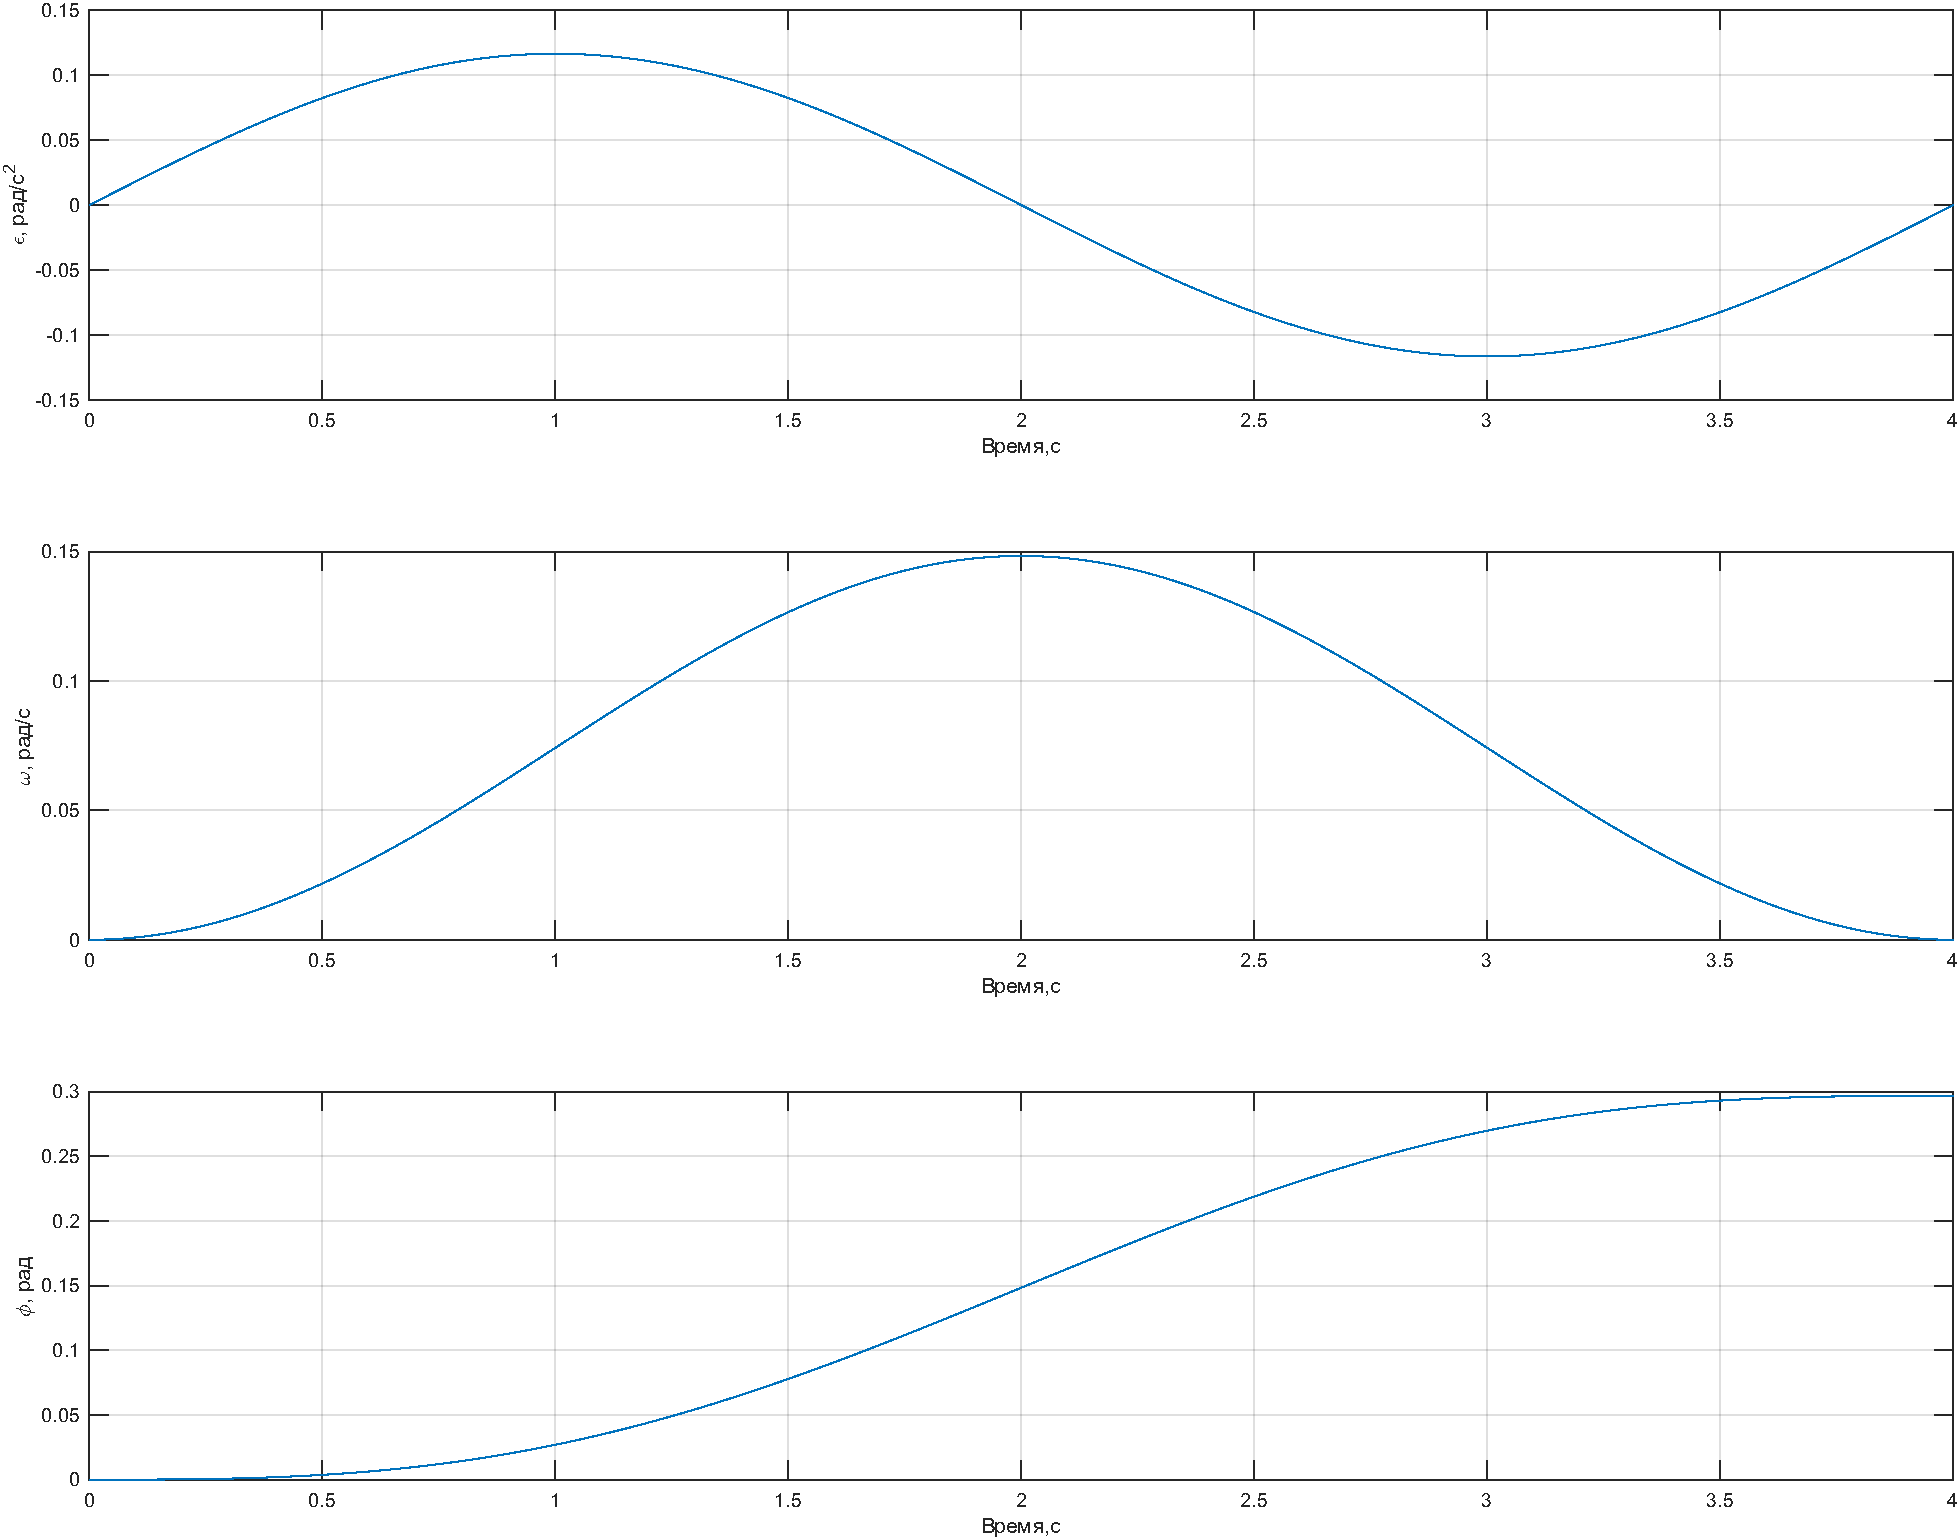
\includegraphics[scale=0.7]{matlab/sin_profile.pdf}}
	\caption{Зависимость углового ускорения, скорости и углового положения от времени}
	\label{fig:sin_profile}
\end{figure}


Таким образом, для задания закона управления приводом достаточно задать значения угла поворота~$\phi$ и времени перемещения~$T$.

На рисунке~\cref{fig:sin_moment} представлен график реактивного момента на основание при моменте инерции блока зеркал $J_m = \SI{2.96}{\kilogram\metre\squared}$.

\begin{figure}[ht]
	\centerfloat{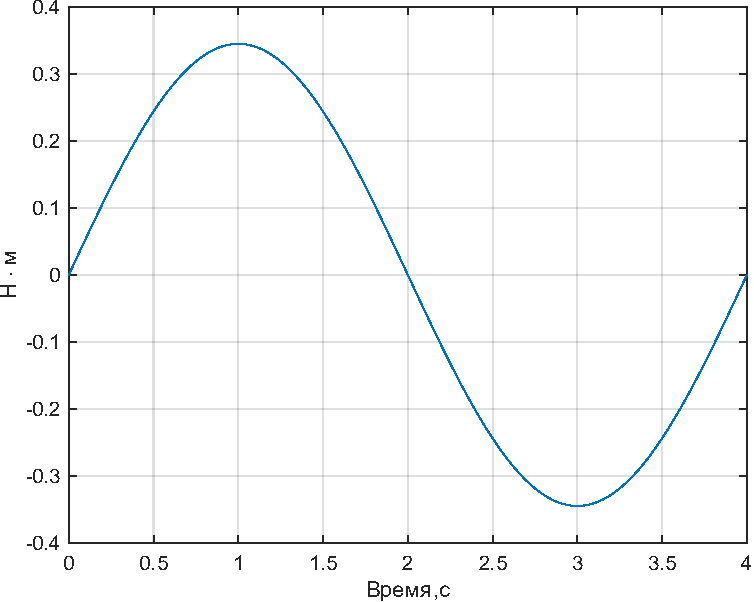
\includegraphics[scale=0.7]{matlab/sin_moment.pdf}}
	\caption{Реактивный момент при синусоидальном профиле разгона}
	\label{fig:sin_moment}
\end{figure}

Из графика видно, что максимальный реактивный момент на основание космического аппарата достигает значения~ $M = J_m \cdot \epsilon = \SI{0.35}{\newton\metre}.$ Момент имеет круговую частоту $f = \frac{\pi}{2}\, \si{\radian/\second}$, что соответствует частоте~\SI{0.25}{\hertz}. Эта частота близка к частотам собственных колебаний космического аппарата: \SI{0.2}{\hertz} по координате~$Z$ и \SI{0.174}{\hertz} по координате~$Y$. Указанное обстоятельство, при плохой настройке маховика и значительных остаточных моментах, может привести к возбуждению колебаний КА по этим осям.

\section{Линейный алгоритм управления}\label{sec:ch2/sec2}

Рассмотрим теперь алгоритм управления по линейному закону.

\begin{figure}[ht]
	\centerfloat{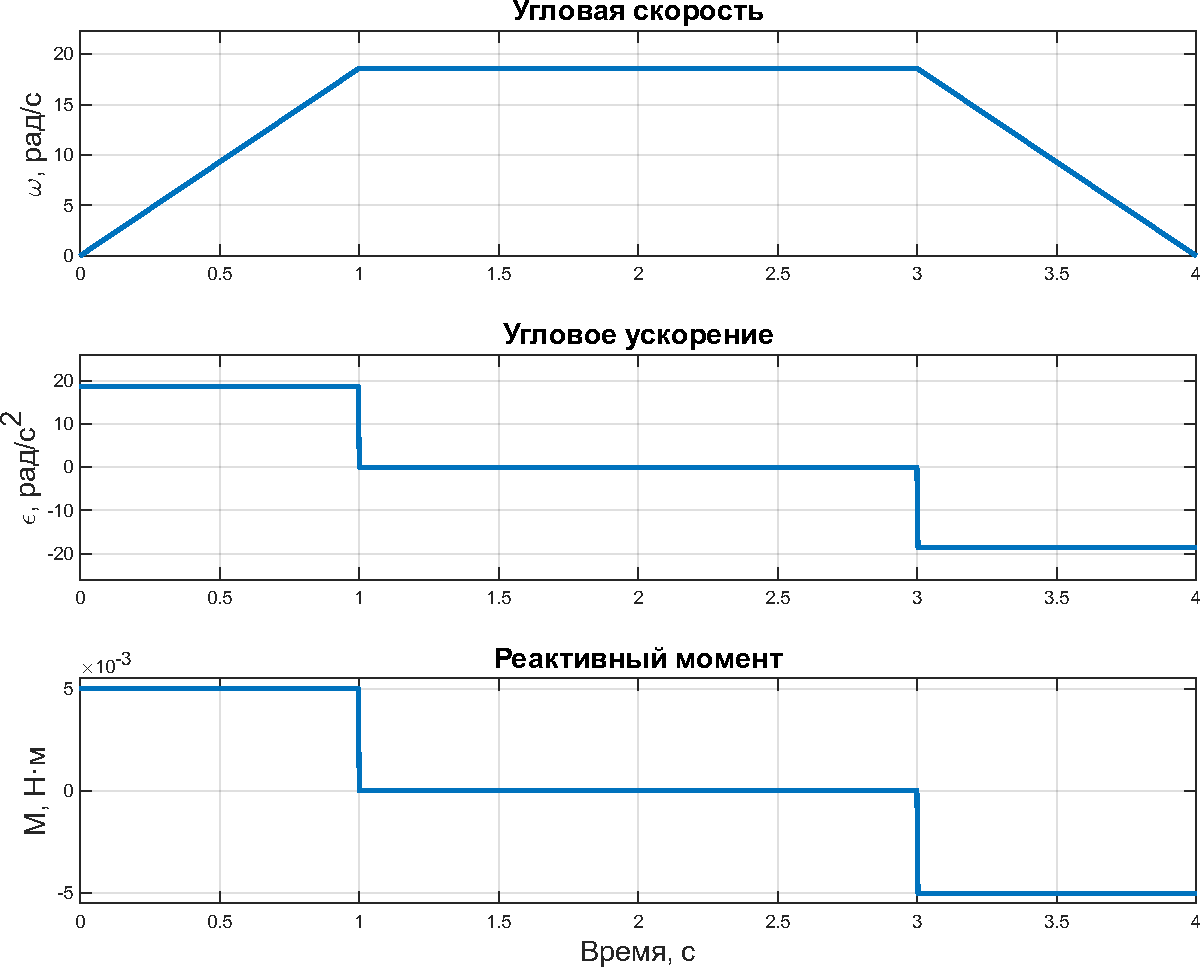
\includegraphics[scale=0.7]{matlab/line_profile.pdf}}
	\caption{Зависимость углового ускорения, скорости и углового положения от времени при линейном профиле разгона}
	\label{fig:line_profile}
\end{figure}

На рисунке~\cref{fig:line_profile} представлен упрощённый график изменения угловой скорости вращения и углового ускорения блока зеркал при перенацеливании на угол 17°. В течение времени разгона $t_a$ происходит увеличение скорости привода СПН, затем в течение $t_n$ происходит  движение с максимальной скоростью, и за время $t_d$ происходит торможение привода. В соответствии с ТЗ весь процесс должен занимать 4 с. Тогда можно записать:

\begin{equation}
	\label{eq:eqCh2_t_move}
	t_a+t_m+t_d=\SI{4}{\second}
\end{equation}

С другой стороны, за это время блок зеркал должен повернуться на угол 17°. Обозначим максимальную скорость $\omega_{nom}$, тогда для угла поворота получим:

\begin{equation}
	\label{eq:eqCh2_t_acc}
	\phi = t_a \cdot \frac{\omega_{nom}}{2} + t_n \cdot \omega_{nom} + t_d \cdot \frac{\omega_{nom}}{2} = \SI{17}{\degree}
\end{equation}

Номинальная скорость определяется из условия, что нужно преодолеть \SI{17}{\degree} за \SI{4}{\second}.
\begin{align*}
	t_a &= t_d = \SI{1}{\second}, \\
	t_n &= \SI{2}{\second}
\end{align*}
Тогда номинальная скорость определяется следующим образом:
\[
\omega_{nom} = \phi / 3 = 0,2967/3 = \SI{0.0989}{\radian/\second} 
\]
Максимальная частота управляющих сигналов для используемого в приводах шагового электродвигателя составляет 500 Гц. Одному периоду сигнала соответствует поворот ротора на угол 1,8°. Таким образом, максимальная скорость вращения шагового электродвигателя составит $\Omega_{d} = 500 \cdot 1,8 = \SI{900} {\degree/ \second}$. Максимальная угловая скорость блока зеркал составит $\Omega_{max}= 900/160 = \SI{5,625}{\degree/ \second}$. Подставим это значение в полученные выше уравнения~\cref{eq:eqCh2_t_move}и~\cref{eq:eqCh2_t_acc} и решим их совместно. Получим:


Отсюда ускорение разгона $\omega_{nom} / t_a = \SI{5,22}{\degree/\second\square} = \SI{0,091}{\radian/\second\square}$


Максимальный (без компенсации маховиками) реактивный момент для момента инерции блока зеркал $J_m = \SI{2,96}{\kilogram\cdot\meter\square}$ будет \mbox{\SI{0,091}{\radian / \second\square}  $\cdot 2,96 = \SI{0,269}{\newton\meter}$}.

Пусть:
\begin{align*}
	t_a &= t_d = \SI{2,05}{\second}, \\
	t_m &= \SI{0}{\second}
\end{align*}

Средняя скорость для выполнения перенацеливания на \SI{17}{\degree}
за \SI{4}{\second} составит $\Omega_{cp} = 17 / 4 = \SI{4,25}{\degree / \second}$. При движении по симметричному треугольному алгоритму ускорение разгона составит $\Omega_{cp} / t_p = \SI{2,024}{\degree / \second\square} = \SI{0,035}{\radian / \second\square}$, тогда максимальный (без компенсации маховиками) реактивный момент для момента инерции зеркал $J_m = \SI{2,96}{\kilogram \cdot \meter\square}$ составит $0,035 \cdot 2,96 = \SI{0,1}{\newton\meter}$

Таким образом, используя линейный треугольный закон разгона-торможения можно снизить реактивный момент на основание в 2,5 раза, что существенно облегчает задачу компенсации реактивного момента.

Следует отметить, что линейный график углового перемещения узла зеркал даёт несколько меньше (по сравнению с синусоидальным законом управления) постоянное значение ускорения (и, соответственно, реактивного момента) на участках разгона и торможения. Таким образом подбирая закон разгона и торможения можно управлять значением реактивного момента.

\section{Экспоненциальный алгоритм управления}\label{sec:ch2/sec3}

Особенности использования шагового электродвигателя со значительной инерционной нагрузкой обуславливают необходимость осуществления его разгона и торможения по определённому закону с плавными изменениями параметров движения. Это позволяет минимизировать вероятность потери шагов, снизить вибрации и обеспечить устойчивую работу привода.

В качестве примера такого закона может быть использована кусочно-заданная функция угловой скорости, включающая три стадии: экспоненциальный разгон, равномерное движение с номинальной скоростью и плавное экспоненциальное торможение. Данный закон описывается следующими выражениями:

\begin{samepage}
\begin{equation}
	\label{eq:expOmega}
	\omega(t) =
	\begin{cases}
		\omega_{\min} + (\omega_{\max} - \omega_{\min}) \cdot \left(1 - e^{-k t} \right),
		& 0 \leq t < t_r \\
		\omega_{\max}, 
		& t_r \leq t < t_r + t_c \\
		\omega_{\min} + (\omega_{\max} - \omega_{\min}) \cdot e^{-k (t - t_r - t_c)},
		& t_r + t_c \leq t \leq T
	\end{cases}
\end{equation}

где: \\
\quad $t$ — время движения; \\
\quad $\Omega(t)$ — угловая скорость во времени; \\
\quad $\Omega_{\min}$, $\Omega_{\max}$ — минимальная и максимальная скорость; \\
\quad $t_a$ — время разгона; \\
\quad $t_n$ — время равномерного движения; \\
\quad $T = 2t_a + t_n$ — общее время движения; \\
\quad $k$ — коэффициент плавности экспоненциального изменения.
\end{samepage}


На рисунке~\ref{fig:exp_profile} приведена характерная S-образная кривая скорости привода, построенная по вышеуказанной формуле. Кривая включает плавный экспоненциальный разгон, участок движения с постоянной скоростью и плавное экспоненциальное торможение.

График построен для случая движения со следующими параметрами: \\
\quad $\Omega_{\max} = 5{,}6^\circ/\text{с}$, \\
\quad $\Omega_{\min} = 0{,}02^\circ/\text{с}$, \\
\quad $k = 4$, \\
\quad $t_r = 1$ с — время разгона, \\
\quad $t_c = 2$ с — время равномерного движения. \\

Использование данной функции позволяет достичь необходимой скорости за ограниченное время с минимальными динамическими нагрузками, что особенно важно при работе с механизмами, обладающими значительным моментом инерции. Кусочно-заданный характер функции обеспечивает плавность переходов между стадиями движения и исключает резкие изменения ускорения, типичные для линейных или трапецеидальных профилей.

\begin{figure}[ht]
	\centerfloat{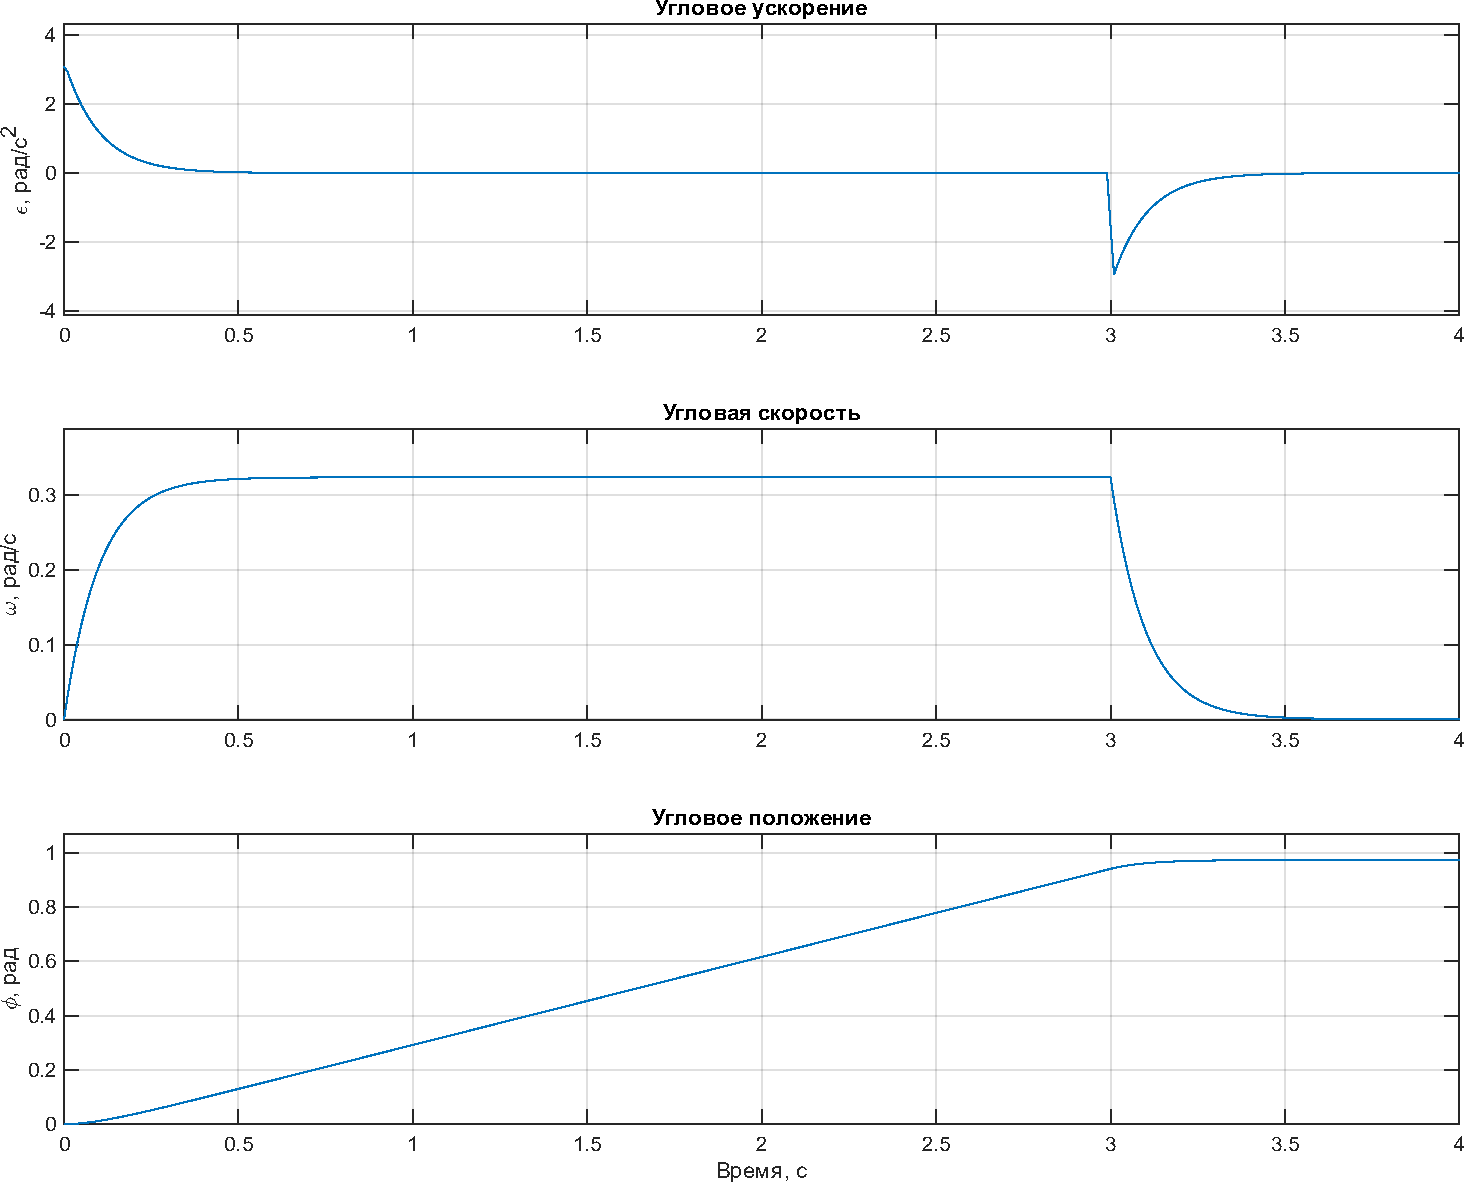
\includegraphics[scale=0.7]{matlab/exp_profile.pdf}}
	\caption{Зависимость углового ускорения, скорости и углового положения от времени при экспоненциальном профиле разгона}
	\label{fig:exp_profile}
\end{figure}

На рисунке~\ref{fig:omega_profile} приведены параметры скорости и ускорения шагового двигателя при разгонах и торможениях, построенная по данной формуле. Она соответствует следующему режиму работы: 
$\Omega_{\max} = 5{,}6 \, \text{°/с}$, 
$\Omega_{\min} = 0{,}02 \, \text{°/с}$, 
$\varepsilon_{\max} = 14 \, \text{°/с}^2 = 0{,}244 \, \text{рад/с}^2$, 
время разгона $t_r = 1 \, \text{с}$, 
длительность равномерного движения $t_c = 2 \, \text{с}$, 
общее время движения $T = 4 \, \text{с}$.


На рисунке приведен также график изменения значения ускорения при разгоне привода. Торможение привода осуществляется по тому же закону, но с зеркальным отражением по отношению к оси времени. Характер изменения возмущающего момента полностью соответствует графику изменения значения ускорения. Установленный в ОС УПК шаговый двигатель развивает момент $\SI{0,9}{\newton\meter}$, чего вполне достаточно для осуществления движения по описанному закону.
Управление приводом перенацеливания по экпоненциальному закону производится в следующем порядке:



\FloatBarrier
